% vim: spell spelllang=en:
%! TEX root = **/00-main.tex

% Additional plots

\section{Additional plots}%
\label{sec:additional_plots}

\newcommand{\centroidmap}[2]{
    \begin{figure}[H]
        \centering
        \includegraphics[width=0.87\linewidth]{pca_fact-plane_#1_#2-cent}
        \caption{PCA plane #1 vs #2 (categorical variables centroids)}%
        \label{fig:plane_#1-#2-cent}
    \end{figure}
}

\begin{landscape}
\centroidmap{1}{2}
\centroidmap{1}{3}
\centroidmap{1}{4}
\centroidmap{2}{3}
\centroidmap{2}{4}
\centroidmap{3}{4}
\end{landscape}

% TODO

% es poden incluir a saco ajuntant els pdfs o amb un bucle o algo.
%\includepdf[pages=-,landscape=true]{../../analysis/plots/PCA_planes_sep}
%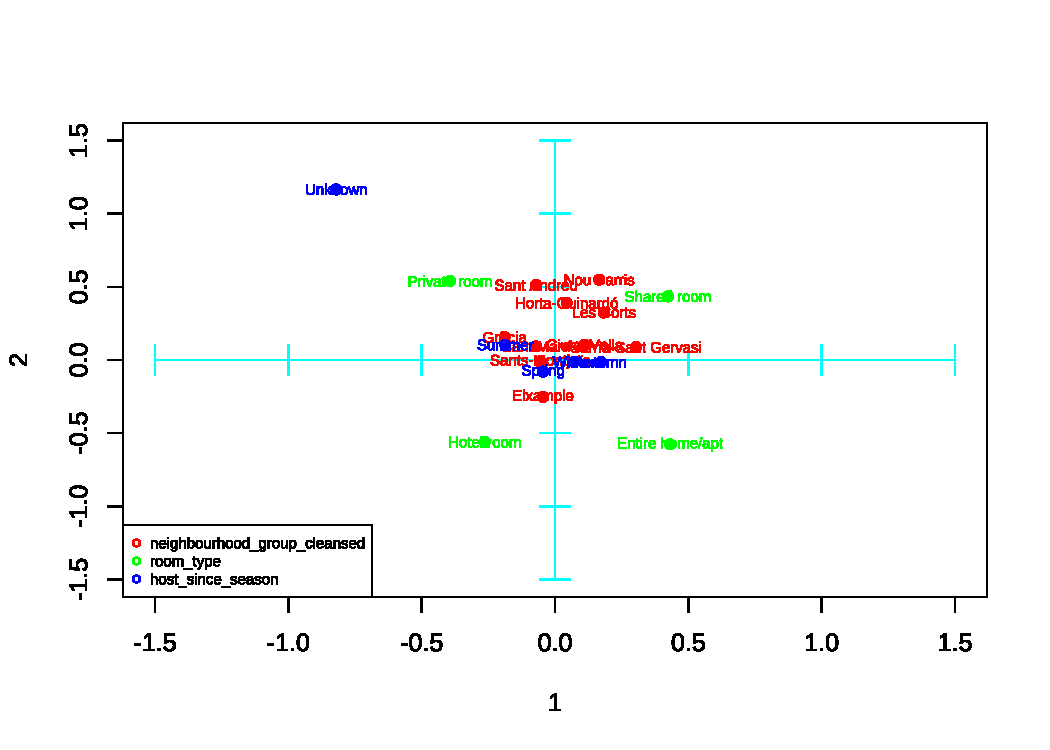
\includepdf[pages=-,landscape=true]{../../analysis/plots/PCA_planes_no_ordi}
%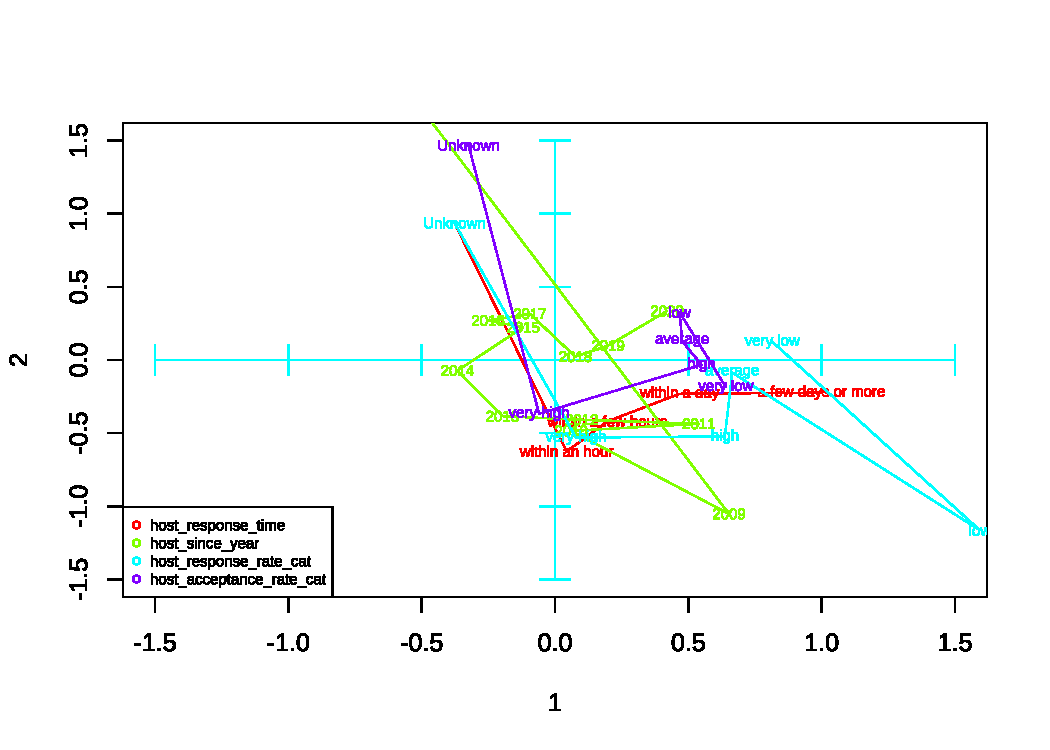
\includepdf[pages=-,landscape=true]{../../analysis/plots/PCA_planes_ordi}
